\section{Giới thiệu}\label{sec:intro}
\frame{\tableofcontents[currentsection]}

\begin{frame}{Giới thiệu}
Định nghĩa bài toán
\begin{itemize}
    \item Là một bài toán tạo sinh dữ liệu dạng hình ảnh dựa trên các dạng dữ liệu khác.
    \item Cho trước một vài dữ liệu về gương mặt của một người bất kỳ \textit{(hình ảnh, video ngắn)} và môt đoạn tiếng nói bất kỳ. Tạo sinh hình ảnh người đó đang nói đoạn tiếng nói đã cho một cách chân thực.
\begin{figure}[H]
    \centering
    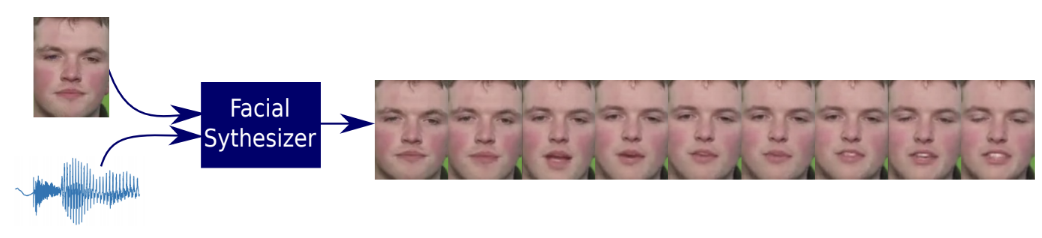
\includegraphics[width=13cm]{images/intro.png}
    \caption{Ví dụ về mô hình tạo sinh khuôn mặt}
    \label{fig:example}
\end{figure}
\end{itemize}
\end{frame}


\begin{frame}{Giới thiệu}
Lý do chọn đề tài
\begin{itemize}
    \item Là nhu cầu cần thiết trong ngành giải trí, phim ảnh, hoạt hình, giúp giảm chi phí sản xuất phim
    \begin{itemize}
        \item Phần hóa trang có thể được cắt bớt
        \item Phần kĩ xảo có thể được đơn giản hóa
    \end{itemize}
    \item Tạo sinh gương mặt đại diện trong trường hợp người nói không muốn lộ diện
    \item Tạo sinh biên tập viên ảo trong chương trình thời sự, dự báo thời tiết
    \item Giả lập trợ lý ảo có hình dáng con người
\end{itemize}
\end{frame}

\begin{frame}{Giới thiệu}
Thách thức
\begin{itemize}
    \item Đây là một đề tài mới lạ, vấn đề tạo sinh dữ liệu chỉ vừa được bùng nổ từ năm 2014 khi mạng GANs xuất hiện
    \item Tạo sinh dữ liệu cũng là một đề tài khó và phức tạp
    \item Tạo sinh video từ những dạng dữ liệu khác (hình ảnh, âm thanh) càng làm cho bài toán trở nên thách thức hơn
    \item Bài toán cũng yêu cầu sức mạnh tính toán lớn và khối lượng dữ liệu lớn
\end{itemize}
\end{frame}

\begin{frame}{Giới thiệu}
\begin{enumerate}
    \item \textit{Mục tiêu}: Xây dựng mô hình có khả năng tạo sinh hình ảnh khuôn mặt người một cách tự nhiên, chính xác.
    \item \textit{Giới hạn}: Tạo sinh hình ảnh trong vùng mặt người. Dữ liệu mẫu được cung cấp ban đầu phải là hình ảnh rõ ràng của khuôn mặt người và một đoạn âm thanh bất kỳ thu âm tiếng nói.
    \item \textit{Đối tượng}: Các phương pháp mô hình hóa bài toán, học máy, học sâu, mạng GANs và các phương pháp tạo sinh dữ liệu từ mạng GANs, các phương pháp kết hợp đặc trưng hình ảnh, âm thanh để tạo sinh dữ liệu mới.
\end{enumerate}
\end{frame}
